% =============================================================================
% handout.tex
% Standalone article-class supplementary handout
% Compile: xelatex handout → biber handout → xelatex handout → xelatex handout
% =============================================================================
\documentclass[11pt,a4paper]{article}
\usepackage[margin=1in]{geometry}
\usepackage{amsmath,amssymb,amsfonts}
\usepackage{booktabs}
\usepackage{graphicx}
\usepackage{array}
\usepackage{tabularx}
\usepackage{float}
\usepackage{hyperref}
\usepackage{xcolor}
\usepackage{csquotes}

\usepackage[backend=biber,style=authoryear,natbib=true,maxcitenames=2,maxbibnames=99]{biblatex}
\addbibresource{slides.bib}

% Match notation from slides
\newcommand{\E}{\mathbb{E}}
\newcommand{\PP}{\mathbb{P}}
\newcommand{\1}{\mathbf{1}}
\newcommand{\Var}{\mathrm{Var}}
\newcommand{\Cov}{\mathrm{Cov}}
\newcommand{\R}{\mathbb{R}}

% Color coding for notation
\definecolor{brightblue}{cmyk}{0.92,0,0.15,0.05}
\newcommand{\choice}[1]{\textcolor{blue}{#1}}
\newcommand{\obs}[1]{\textcolor{red!70!black}{#1}}
\newcommand{\outcome}[1]{\textcolor{green!50!black}{#1}}

\graphicspath{{../numerical_output/}}

\title{\textbf{Liquidity, Activism Disclosure, and Takeover Premia}\\[0.3em]
\large Supplementary Handout}
\author{Austin Li\\University College London}
\date{}

\begin{document}
\maketitle

% =============================================================================
\section{Model Summary}
% =============================================================================

\subsection{Notation}

Table~\ref{tab:notation} collects the full notation used in the model.
Color coding distinguishes \choice{choices} made by agents,
\obs{observables} available to the market, and
\outcome{outcomes} determined in equilibrium.

\begin{table}[H]
\centering
\small
\caption{Model notation. \choice{Blue}: agent choices.
  \obs{Red}: observables. \outcome{Green}: equilibrium outcomes.}
\label{tab:notation}
\begin{tabularx}{\textwidth}{@{}l l X@{}}
\toprule
\textbf{Symbol} & \textbf{Type} & \textbf{Description} \\
\midrule
\multicolumn{3}{@{}l}{\textit{Choices / Actions}} \\[2pt]
\choice{$q \in \{-1,0,+1\}$}
  & Trade quantity & Sell ($-1$), hold ($0$), or buy ($+1$) \\
\choice{$a \in \{0,1\}$}
  & Engagement & Inactive ($0$) or engage ($1$) \\
$z \in \{-1,0,+1\}$
  & Noise trade & Exogenous noise trader order \\[4pt]
\multicolumn{3}{@{}l}{\textit{Observables}} \\[2pt]
\obs{$X = q + z$}
  & Order flow & Aggregate order flow observed by market maker \\
\obs{$D = \1\{q = +1\}$}
  & Disclosure & Public filing triggered by net purchase \\
$s$
  & Signal & Blockholder's private signal, $s = v + \varepsilon$ \\
$v$
  & Fundamental & Firm value, $v \sim N(\mu, \sigma_v^2)$ \\[4pt]
\multicolumn{3}{@{}l}{\textit{Equilibrium Outcomes}} \\[2pt]
\outcome{$P(X,D)$}
  & Price & Market-clearing price \\
\outcome{$\pi(X,D)$}
  & Posterior & $\PP(\text{engaged} \mid X, D)$ \\
\outcome{$p(P,D)$}
  & Bid probability & Prob.\ of takeover bid arrival \\
\outcome{$m(X,D)$}
  & Premium & Expected takeover premium, $m_0 + (\tilde{m} - m_0)\pi(X,D)$ \\[4pt]
\multicolumn{3}{@{}l}{\textit{Parameters}} \\[2pt]
$\kappa$
  & Liquidity & Noise trading intensity; $z = 0$ with prob $1-\kappa$ \\
$k_1, k_0, k_D$
  & Cutoffs & Exit/Hold, Hold/Quiet, Quiet/Public boundaries \\
$\rho$
  & Success prob. & Prob.\ engagement succeeds (value improvement and premium wedge realized) \\
$m_0, m_1$
  & Premia & Baseline premium $m_0$ and premium if engagement succeeds $m_1$ \\
$\tilde{m}$
  & Expected premium & Expected premium under engagement, $\tilde{m} = m_0 + \rho(m_1 - m_0)$ \\
$\Delta, \tilde{\Delta}$
  & Value-add & Standalone improvement if successful; $\tilde{\Delta} = \rho \Delta$ \\
$C_0, \chi$
  & Cost & Engagement cost scale and signal sensitivity \\
\bottomrule
\end{tabularx}
\end{table}

\subsection{Timeline}

The model unfolds in four stages:

\begin{description}
\item[$t=0$ (Nature)] Firm fundamental $v \sim N(\mu, \sigma_v^2)$ is drawn.
  The blockholder observes a private signal $s = v + \varepsilon$
  with $\varepsilon \sim N(0, \sigma_\varepsilon^2)$.
  The noise trader's order $z$ is drawn from $\{-1, 0, +1\}$
  with probabilities $(\kappa/2,\; 1-\kappa,\; \kappa/2)$.

\item[$t=1$ (Trading)] The blockholder chooses $(q, a)$:
  trade quantity $q \in \{-1, 0, +1\}$ and engagement $a \in \{0, 1\}$.
  The market maker observes the public signal $(X, D)$ where
  $X = q + z$ is aggregate order flow and $D = \1\{q = +1\}$
  is a disclosure indicator.

\item[$t=1.5$ (Bidder Entry)] A potential acquirer draws a private
  synergy shock $\xi$ and decides whether to bid.
  The bid probability depends on the price and expected premium:
  $p(P, D) = 1 - \Phi\bigl((m(X,D) + K - \bar{S} + P) / \sigma_\xi\bigr)$.

\item[$t=2$ (Payoffs)] If a bid arrives, the takeover occurs at
  price $P + m(X,D)$. If engagement succeeded ($a=1$, success probability
  $\rho$), the premium is $m_1$ rather than $m_0$, and the fundamental
  improves by $\Delta$.
\end{description}

\subsection{Key Assumptions}

\begin{enumerate}
\item \textbf{Discrete trading.} The blockholder's trade $q \in \{-1, 0, +1\}$
  is a discrete unit trade, following \citet{BackEtAl2018}.
\item \textbf{Noise structure.} The noise trader's order
  $z \in \{-1, 0, +1\}$ is symmetric with intensity $\kappa$.
\item \textbf{Disclosure rule.} Net purchases ($q=+1$) trigger a mandatory
  public filing ($D=1$); sales and holds do not.
\item \textbf{Engagement cost.} Private engagement costs
  $C(s) = C_0 \exp(-\chi\, (s - \mu)/\sigma_s)$ decrease with the signal,
  so better-informed blockholders find it cheaper to engage.
\item \textbf{Bidder entry.} The acquirer's entry decision depends on the
  market price through a feedback channel: higher prices raise the cost
  of acquisition, reducing bid probability.
\end{enumerate}

\subsection{Action Space}

The blockholder's four actions are combinations of trading and engagement:

\begin{table}[H]
\centering
\caption{Blockholder action space.}
\label{tab:actions}
\begin{tabular}{@{}lcc@{}}
\toprule
\textbf{Action} & \textbf{Trade $q$} & \textbf{Engage $a$} \\
\midrule
Exit         & $-1$ & $0$ \\
Hold         & $0$  & $0$ \\
Quiet Voice  & $0$  & $1$ \\
Public Voice & $+1$ & $1$ \\
\bottomrule
\end{tabular}
\end{table}


% =============================================================================
\section{Equilibrium Characterization}
% =============================================================================

\subsection{Proposition 1: Monotone Cutoff Equilibrium}

\textbf{Statement.}
In equilibrium, the blockholder's strategy is characterized by three
signal cutoffs $k_1 \leq k_0 \leq k_D$ such that:
\[
(q, a) =
\begin{cases}
(-1, 0) \quad \text{Exit}         & \text{if } s < k_1 \\
(0, 0)  \quad \text{Hold}         & \text{if } k_1 \leq s < k_0 \\
(0, 1)  \quad \text{Quiet Voice}  & \text{if } k_0 \leq s < k_D \\
(+1, 1) \quad \text{Public Voice} & \text{if } s \geq k_D
\end{cases}
\]

\textit{Proof sketch.}
Single-crossing: each action's expected payoff has a steeper slope in $s$
than the action below it. Exit payoff decreases most slowly in $s$ (sells
into a low signal), while Public Voice payoff increases most steeply
(buys and engages when the signal is high). Incentive compatibility at
each boundary pins down the three cutoffs.

Under the baseline calibration, the Hold region collapses
($k_1 = k_0 \approx 0.82$), so the blockholder transitions directly
from Exit to Quiet Voice.

\subsection{Proposition 2: Bayesian Posteriors}

The market's posterior probability that the blockholder is engaged,
$\pi(X, D) = \PP(\text{engaged} \mid X, D)$, has two branches:

\textbf{Disclosure branch ($D=1$).}
Disclosure reveals $q = +1$, which implies $a = 1$ (Public Voice).
Therefore $\pi(X, 1) = 1$ for all $X \in \{0, 1, 2\}$.

\textbf{No-disclosure branch ($D=0$).}
For $X \in \{-2, -1, 0, 1\}$, define the action probabilities:
\begin{align}
  \omega_E &= \Phi\!\left(\frac{k_1 - \mu}{\sigma_s}\right),
  &
  \omega_H &= \Phi\!\left(\frac{k_0 - \mu}{\sigma_s}\right) - \omega_E,
  \\
  \omega_Q &= \Phi\!\left(\frac{k_D - \mu}{\sigma_s}\right)
    - \Phi\!\left(\frac{k_0 - \mu}{\sigma_s}\right),
  &
  \omega_P &= 1 - \Phi\!\left(\frac{k_D - \mu}{\sigma_s}\right),
\end{align}
and the noise probabilities $p_0 = 1 - \kappa$, $p_1 = \kappa/2$.
Then:
\begin{align}
  \pi(-1, 0) &= \frac{\omega_Q \cdot p_1}
    {(\omega_H + \omega_Q) \cdot p_1 + \omega_E \cdot p_0}, \\[4pt]
  \pi(0, 0) &= \frac{\omega_Q \cdot p_0}
    {(\omega_H + \omega_Q) \cdot p_0 + \omega_E \cdot p_1}, \\[4pt]
  \pi(1, 0) &= \frac{\omega_Q \cdot p_1}
    {\omega_H \cdot p_1 + \omega_Q \cdot p_1}
    = \frac{\omega_Q}{\omega_H + \omega_Q}.
\end{align}

Note that $\pi(1,0)$ does \emph{not} depend on $\kappa$; it is
determined purely by the relative probabilities of Hold and Quiet Voice
generating $X=1$ (both require $z = +1$, so the noise probability cancels).

\subsection{Proposition 3: Price Fixed Point}

The equilibrium price satisfies the fixed-point equation:
\[
P(X,D) = \delta \bigl[ (1 - p^*) \hat{V}(X,D) + p^* (P(X,D) + m(X,D)) \bigr],
\]
where $p^* = p(P(X,D), D)$ is the equilibrium bid probability,
$\hat{V}(X,D) = \E[v \mid X, D] + \tilde{\Delta} \cdot \pi(X,D)$
is the standalone value under expected engagement improvement, and
$m(X,D) = m_0 + (\tilde{m} - m_0)\pi(X,D)$ is the expected premium.

The bid probability depends on the price:
\[
p(P, D) = 1 - \Phi\!\left(\frac{m(X,D) + K - \bar{S} + P}{\sigma_\xi}\right).
\]

A contraction mapping argument guarantees existence and uniqueness of
the fixed point under regularity conditions on $\delta$.

\textbf{Economic interpretation.}
The price reflects a weighted average of the standalone value
(if no bid arrives) and the takeover value (if a bid arrives).
Because a higher price discourages bidder entry, there is a negative
feedback loop: prices partially self-correct, preventing extreme
overvaluation.

\subsection{Proposition 4: Non-Monotone Liquidity Effect}

\textbf{Statement.}
The expected minority takeover gains
$\Delta^{\min}(\kappa)$ are hump-shaped in liquidity $\kappa$.

\textbf{Two opposing forces:}
\begin{enumerate}
\item \textbf{Bid incidence effect} (rising in $\kappa$).
  Higher liquidity provides more camouflage, enabling Quiet Voice
  engagement, which raises posteriors $\pi$ and bid probabilities.
\item \textbf{Inference quality effect} (falling in $\kappa$).
  Higher liquidity adds noise, diluting the market's ability to
  distinguish engaged from non-engaged blockholders, compressing
  posteriors toward the prior.
\end{enumerate}

At low $\kappa$, the first effect dominates; at high $\kappa$, the
second dominates. The peak occurs at an interior $\kappa^*$.


% =============================================================================
\section{Posterior Formulas}
% =============================================================================

\textbf{Disclosure ($D=1$).}
Disclosure requires $q = +1$, which only occurs under Public Voice.
The posterior is trivially $\pi(X, 1) = 1$. Order flow $X \in \{0,1,2\}$
refines information about $z$ but not about engagement.

\textbf{No disclosure ($D=0$).}
The key inference problem: conditional on $D=0$, the blockholder
chose Exit ($q=-1$), Hold ($q=0$), or Quiet Voice ($q=0$, $a=1$).
For each order flow realization $X$, the market updates using Bayes' rule.

\textit{Why $\pi(1, 0)$ is independent of $\kappa$.}
When $X = 1$ and $D = 0$, the blockholder did not buy ($q \neq +1$).
So $X = 1$ requires $z = +1$ regardless of the blockholder's action.
The only actions compatible with $q \leq 0$ and $X = 1$ are Hold
($q=0, z=+1$) and Quiet Voice ($q=0, z=+1$). Both require the same
noise realization $z=+1$, so $\kappa$ cancels from the likelihood ratio:
\[
\pi(1,0) = \frac{\omega_Q \cdot p_1}{\omega_H \cdot p_1 + \omega_Q \cdot p_1}
  = \frac{\omega_Q}{\omega_H + \omega_Q}.
\]


% =============================================================================
\section{Pricing Equation}
% =============================================================================

\subsection{Fixed-Point Structure}

The price $P(X,D)$ satisfies:
\begin{equation}\label{eq:price-fp}
P = \delta \Bigl[
  \bigl(1 - p(P,D)\bigr)\,\hat{V}(X,D)
  + p(P,D)\,\bigl(P + m(X,D)\bigr)
\Bigr].
\end{equation}

\textbf{Components:}
\begin{itemize}
\item \textbf{Standalone value:}
  $\hat{V}(X,D) = \E[v \mid X, D] + \tilde{\Delta}\, \pi(X,D)$
  reflects the fundamental conditional on the information set plus the
  expected value improvement from engagement.

\item \textbf{Bid probability:}
  \begin{equation}\label{eq:bid-prob}
    p(P, D) = 1 - \Phi\!\left(
      \frac{m(X,D) + K - \bar{S} + P}{\sigma_\xi}
    \right).
  \end{equation}
  Since $P(\cdot,D)$ is injective (Assumption A7), the bidder infers $X$ from $P$; we write $m(X,D)$ as shorthand.

  A higher price raises the effective acquisition cost,
  reducing the probability that the bidder's synergy shock exceeds
  the entry threshold.

\item \textbf{Expected premium:}
  $m(X,D) = m_0 + (\tilde{m} - m_0)\,\pi(X,D)$.
  Ranges from $m_0$ (no engagement) to $\tilde{m}$ (certain engagement, $\pi=1$).
\end{itemize}

\subsection{Regularity and Contraction}

Equation~\eqref{eq:price-fp} defines $P$ as a fixed point of a map
$T(P)$. The derivative $T'(P)$ involves $\delta$ and the
density $\phi(\cdot)$ evaluated at the bid threshold. A sufficient
condition for contraction ($|T'(P)| < 1$) restricts
$\delta$ to ensure the feedback loop is not explosive. Under the
baseline calibration, $T'(P) \approx 0.4$, so convergence is rapid.


% =============================================================================
\section{Numerical Calibration}
% =============================================================================

\subsection{Parameter Values}

Table~\ref{tab:calibration} reports the baseline calibration.

\begin{table}[H]
\centering
\caption{Baseline parameter calibration.}
\label{tab:calibration}
\begin{tabular}{@{}llrl@{}}
\toprule
\textbf{Parameter} & \textbf{Symbol} & \textbf{Value} & \textbf{Description} \\
\midrule
Discount factor         & $\delta$        & 0.95  & Time value of money \\
Liquidity               & $\kappa$        & 0.50  & Noise trading intensity \\
Prior mean              & $\mu$           & 1.00  & Mean fundamental value \\
Fundamental std         & $\sigma_v$      & 0.50  & Uncertainty in $v$ \\
Signal noise std        & $\sigma_\varepsilon$ & 0.50  & Noise in private signal \\
Engagement cost scale   & $C_0$           & 0.12  & Base cost of engagement \\
Cost sensitivity        & $\chi$          & 0.50  & Signal sensitivity of cost \\
Success probability     & $\rho$          & 0.90  & Prob.\ engagement succeeds \\
Engagement value-add    & $\Delta$        & 0.25  & Value improvement \\
Base premium            & $m_0$           & 0.10  & Premium without engagement \\
Success premium         & $m_1$           & 0.30  & Premium with successful engagement \\
Baseline synergy        & $\bar{S}$       & 1.44  & Mean synergy for bidder \\
Entry cost              & $K$             & 0.15  & Bidding cost \\
Synergy shock std       & $\sigma_\xi$    & 0.40  & Volatility of synergy shock \\
\bottomrule
\end{tabular}
\end{table}

\subsection{Baseline Equilibrium}

Under the baseline calibration, the equilibrium cutoffs are
$k_1 = k_0 \approx 0.82$ and $k_D \approx 2.26$.
The Hold region collapses ($k_1 = k_0$): the blockholder transitions
directly from Exit to Quiet Voice. Public Voice is triggered only
for very high signals ($s \geq k_D$).

Table~\ref{tab:baseline} reports the full equilibrium price schedule.

\begin{table}[H]
\centering
\caption{Baseline equilibrium: prices, posteriors, bid probabilities,
  and premia across information sets $(X, D)$.}
\label{tab:baseline}
\begin{tabular}{llrrrr}
\toprule
$D$ & Order flow $X$ & $P(X,D)$ & $\pi(X,D)$ & $p(X,D)$ & $m(X,D)$ \\
\midrule
0 & $-2$ & 0.84 & 0.00 & 0.81 & 0.10 \\
0 & $-1$ & 1.06 & 0.41 & 0.55 & 0.17 \\
0 & $0$ & 1.23 & 0.74 & 0.33 & 0.23 \\
0 & $1$ & 1.39 & 1.00 & 0.17 & 0.28 \\
\midrule
1 & $0$ & 1.90 & 1.00 & 0.01 & 0.28 \\
1 & $1$ & 1.90 & 1.00 & 0.01 & 0.28 \\
1 & $2$ & 1.90 & 1.00 & 0.01 & 0.28 \\
\bottomrule
\end{tabular}

\end{table}


% =============================================================================
\section{Figures}
% =============================================================================

\begin{figure}[H]
\centering

\includegraphics[width=0.85\textwidth]{fig_cutoff_structure.pdf}
\caption{\textbf{Equilibrium Cutoff Structure.}
  Action regions in signal space. The blockholder exits for
  $s < k_1$, holds for $k_1 \leq s < k_0$ (region collapses under
  baseline calibration), engages quietly for $k_0 \leq s < k_D$,
  and engages publicly for $s \geq k_D$. Cutoff locations are
  determined by incentive compatibility at each boundary.}
\label{fig:cutoffs}
\end{figure}

\begin{figure}[H]
\centering

\includegraphics[width=0.85\textwidth]{fig_nonmonotone.pdf}
\caption{\textbf{Non-Monotone Liquidity Effect.}
  Expected minority takeover gains $\Delta^{\min}$ as a function
  of liquidity $\kappa$. The hump shape reflects two opposing forces:
  higher liquidity enables camouflaged engagement (raising gains at
  low $\kappa$) but dilutes information quality (reducing gains at
  high $\kappa$). The peak occurs at an interior $\kappa^*$.}
\label{fig:nonmonotone}
\end{figure}

\begin{figure}[H]
\centering

\includegraphics[width=0.85\textwidth]{fig_decomposition.pdf}
\caption{\textbf{Decomposition of Minority Gains.}
  Base premium component $m_0 \cdot \Pr(\text{bid})$ versus
  activism component $\Delta^{\text{act}}$. The base component
  captures gains available to any minority shareholder; the activism
  component reflects additional gains from the blockholder's engagement
  activity and its effect on takeover premia.}
\label{fig:decomposition}
\end{figure}

\begin{figure}[H]
\centering
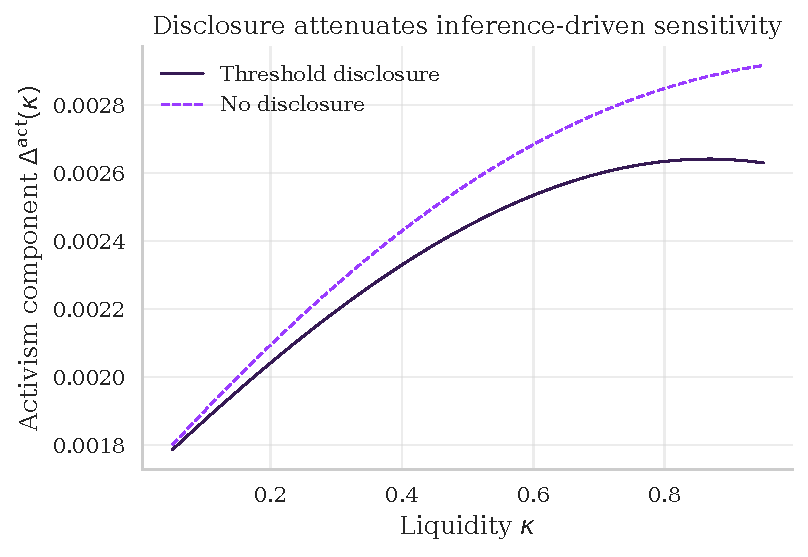
\includegraphics[width=0.85\textwidth]{fig_disclosure.pdf}
\caption{\textbf{Disclosure Attenuation.}
  Comparison of expected minority gains across disclosure states.
  Disclosure ($D=1$) fully reveals engagement, eliminating the
  information asymmetry. The gap between $D=0$ and $D=1$ outcomes
  quantifies the information value of the disclosure channel.}
\label{fig:disclosure}
\end{figure}

\begin{figure}[H]
\centering

\includegraphics[width=0.85\textwidth]{fig_cutoffs_kappa.pdf}
\caption{\textbf{Cutoffs vs.\ Liquidity.}
  How equilibrium boundaries $k_1$, $k_0$, and $k_D$ shift with
  liquidity $\kappa$. As $\kappa$ increases, the noise cover expands
  the Quiet Voice region and shifts the Public Voice boundary.}
\label{fig:cutoffs-kappa}
\end{figure}

\begin{figure}[H]
\centering

\includegraphics[width=0.85\textwidth]{fig_prices.pdf}
\caption{\textbf{Price Function.}
  Equilibrium prices $P(X,D)$ across all information sets.
  Prices are increasing in order flow $X$ and in the disclosure
  indicator $D$, reflecting the market's Bayesian updating about
  engagement and fundamental value.}
\label{fig:prices}
\end{figure}

\begin{figure}[H]
\centering

\includegraphics[width=0.85\textwidth]{fig_sensitivity_C0.pdf}
\caption{\textbf{Sensitivity to Engagement Cost.}
  Effect of varying $C_0$ on minority gains. Higher engagement
  costs shrink the Quiet Voice region, reducing activism-driven
  gains. Below a threshold $C_0$, engagement is nearly costless
  and the blockholder engages for almost all positive signals.}
\label{fig:sensitivity-C0}
\end{figure}

\begin{figure}[H]
\centering

\includegraphics[width=0.85\textwidth]{fig_sensitivity_wedge.pdf}
\caption{\textbf{Sensitivity to Resistance Wedge.}
  Effect of varying the premium gap $m_1 - m_0$ on minority gains.
  A larger wedge increases the return to engagement, expanding the
  Voice region and amplifying the non-monotone liquidity effect.
  When $m_1 = m_0$, the activism channel shuts down entirely.}
\label{fig:sensitivity-wedge}
\end{figure}


% =============================================================================
\section{Extensions: Alternative Disclosure Regimes}
% =============================================================================

The baseline model features a mandatory disclosure rule where net
purchases trigger a public filing. Three alternative regimes illustrate
how disclosure design interacts with blockholder incentives:

\begin{description}
\item[FI (Full Information):] The signal $S = (q, a)$ fully reveals the
  blockholder's action. Inference is shut down: $\pi_{\text{FI}} = 1$
  if $a=1$ and $\pi_{\text{FI}} = 0$ if $a=0$. This eliminates the
  strategic interaction between trading and engagement but allows the
  market to perfectly price the fundamental.

\item[ND (No Disclosure):] The signal $S = \varnothing$ reveals nothing
  beyond order flow. Engagement must be inferred from $X$ alone in all
  states. Quiet Voice and Public Voice become indistinguishable
  conditional on the same $X$, weakening incentives to buy when
  engaging.

\item[NR (Noisy Rumor):] The signal $S = (D, R)$ augments the
  disclosure indicator with a noisy rumor $R$ that is informative
  about quiet engagement. This partially bridges the gap between
  the baseline and full information regimes.
\end{description}

Table~\ref{tab:extensions} compares posteriors across regimes.

\begin{table}[H]
\centering
\caption{Posterior comparison across disclosure regimes.}
\label{tab:extensions}
\begin{tabular}{lrrrr}
\toprule
$X$ & $\pi(X,0)$ & $\pi_{\textup{ND}}(X)$ & $\pi_{\textup{NR}}(X,0,R=0)$ & $\pi_{\textup{NR}}(X,0,R=1)$ \\
\midrule
$-1$ & 0.41 & 0.41 & 0.19 & 0.68 \\
$0$ & 0.74 & 0.74 & 0.48 & 0.89 \\
$1$ & 1.00 & 1.00 & 1.00 & 1.00 \\
\bottomrule
\end{tabular}
\vspace{0.6em}
\begin{tabular}{ll}
\toprule
$(q,a)$ & $\pi_{\textup{FI}}$ \\
\midrule
$(-1,0)$ & 0.00 \\
$(0,0)$ & 0.00 \\
$(0,1)$ & 1.00 \\
$(1,1)$ & 1.00 \\
\bottomrule
\end{tabular}

\end{table}


% =============================================================================
\printbibliography
% =============================================================================

\end{document}
